
In this Appendix, I plot the time course analyses
for Experiment 6, reported in Chapter 6,
separately for each of the eight CRT problems.
The text of the conflict and no-conflict versions
of the eight items are shown in Appendix~\ref{appendix:exp6_stimuli}.

For clarity, I use labels to refer to each CRT problems.
Therefore, problems 1, 2, and 3 in Appendix~\ref{appendix:exp6_stimuli}
\citep[the original CRT items, from][]{Frederick2005} will be referred to as
the \emph{bat-and-ball}, \emph{widgets}, and \emph{lily pad} problems respectively.
Similarly, problems 5 -- 8, adapted from \citet{Primi2015},
will be referred to the
\emph{coin} (4),
\emph{elves} (5),
\emph{running track} (6),
\emph{grades} (7),
and \emph{athletics team} (8)
problems.


\begin{figure}[h]
  \centering
  \includegraphics[width=.9\textwidth]{imgs/exp6/all_items.pdf}
  %% \caption[Proportion of mouse cursors in each responses' region of the screen over time,
  %% seperately for each problem, Experiment 6.]{
  \caption[]{
    Proportion of mouse cursors in the region of the screen 
    corresponding to each response options, over time, 
    for conflict and no-conflict problems,
    separately for each CRT problem
    (see also Figure~\ref{fig:exp6-all}).
  }
\end{figure}

\begin{figure}[h]
  \centering
  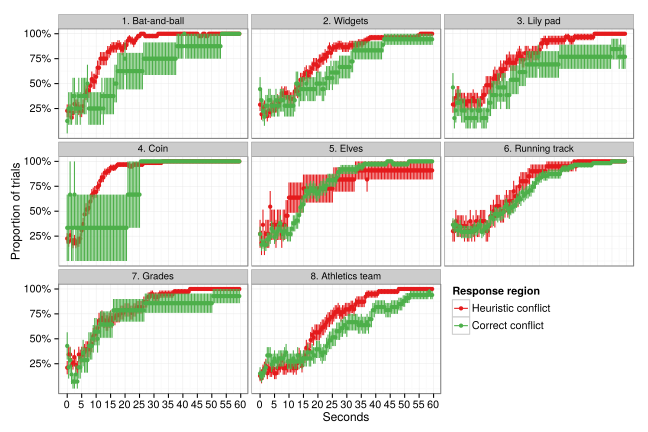
\includegraphics[width=.9\textwidth]{imgs/exp6/conflict-to-chosen_items.pdf}
  %% \caption[Proportion of cursors in region of chosen option,
  %% on conflict problems,
  %% seperately for each problem, Experiment 6.]{
  \caption[]{
    Proportion of mouse cursors in the region of
    the response option which was ultimately selected on that trial,
    comparing movements to the heuristic and correct options on conflict problems,
    separately for each CRT problem
    (see also Figure~\ref{fig:exp6-all-to-chosen}).
  }
\end{figure}

\begin{figure}[h]
  \centering
  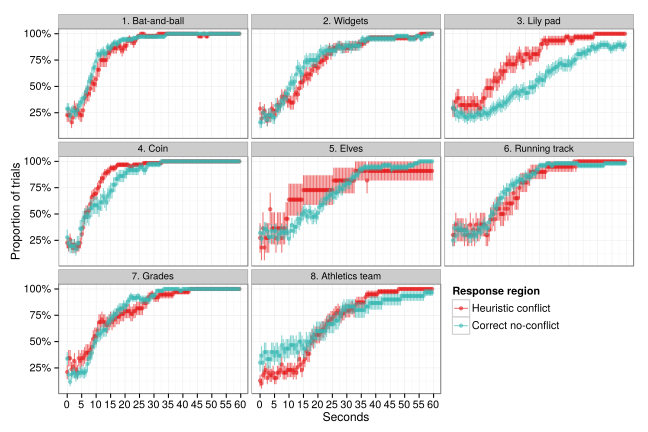
\includegraphics[width=.9\textwidth]{imgs/exp6/intuitive-to-chosen_items.pdf}
  %% \caption[Proportion of cursors in region of chosen option,
  %% for heuristically-cued responses,
  %% seperately for each problem, Experiment 6.]{
  \caption[]{
    Proportion of mouse cursors in the region of
    the response option which was ultimately selected on that trial,
    comparing movements to the heuristic option conflict problems
    to those to the correct options on no-conflict problems,
    separately for each CRT problem
    (see also Figure~\ref{fig:exp6-all-to-chosen}).
    \label{fig:exp6-heuristic-to-chosen-by-item}
  }
\end{figure}


\begin{figure}[h]
  \centering
  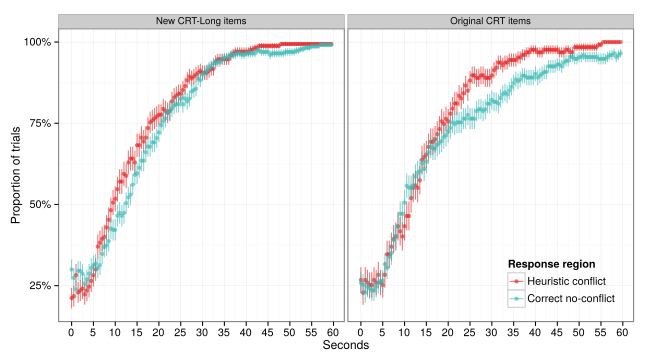
\includegraphics[width=.9\textwidth]{imgs/exp6/intuitive-to-chosen_oldnew.pdf}
  %% \caption[Proportion of cursors in region of chosen option,
  %% for heuristically-cued responses,
  %% seperately for original and extended CRT problems, Experiment 6.]{
  \caption[]{
    Proportion of mouse cursors in the region of
    the response option which was ultimately selected on that trial,
    comparing movements to the heuristic option conflict problems
    to those to the correct options on no-conflict problems,
    separately for the original problems adapted from \citet{Frederick2005},
    and the problems adapted from \citet{Primi2015}
    (see also Figure~\ref{fig:exp6-all-to-chosen}).
  }
\end{figure}




\begin{figure}[h]
  \centering
  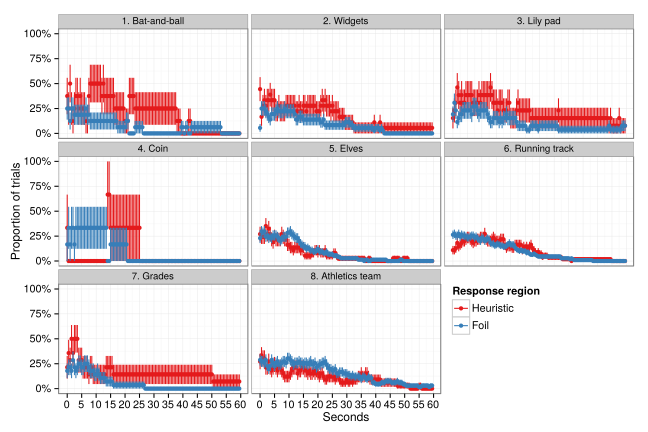
\includegraphics[width=.9\textwidth]{imgs/exp6/correct-not-chosen_items.pdf}
  %% \caption[Proportion of cursor in region of other response options
  %%   when correct response was given,
  %%   seperately for each problem, Experiment 6.]{
  \caption[]{
    Proportion of trials in the region of each option, over time,
    for trials in which the correct option was eventually chosen,
    separately for each CRT problem
    (see also Figure~\ref{fig:exp6-correct-not-chosen}).
    Error bars show standard error of measurement.
  }
\end{figure}

\begin{figure}[h]
  \centering
  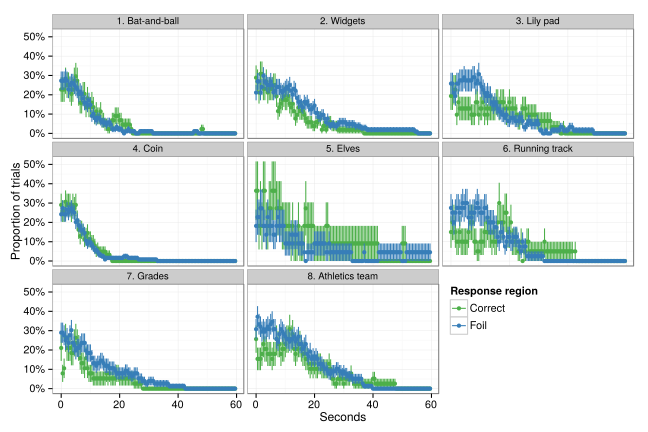
\includegraphics[width=.9\textwidth]{imgs/exp6/heuristic-not-chosen_items.pdf}
  %% \caption[Proportion of cursor in region of other response options
  %%   when heuristic response was given,
  %%   seperately for each problem, Experiment 6.]{
  \caption[]{
    Proportion of trials in the region of each option, over time,
    for trials in which the intuitive option was eventually chosen,
    separately for each CRT problem
    (see also Figure~\ref{fig:exp6-heuristic-not-chosen}).
  }
\end{figure}
